%%%%%%%%%%%%%%%%%%%%%%%%%%%%%%%%%%%%%%%%%
% baposter Landscape Poster
% LaTeX Template
% Version 1.0 (11/06/13)
%
% baposter Class Created by:
% Brian Amberg (baposter@brian-amberg.de)
%
% This template has been downloaded from:
% http://www.LaTeXTemplates.com
%
% License:
% CC BY-NC-SA 3.0 (http://creativecommons.org/licenses/by-nc-sa/3.0/)
%
%%%%%%%%%%%%%%%%%%%%%%%%%%%%%%%%%%%%%%%%%

%----------------------------------------------------------------------------------------
%	PACKAGES AND OTHER DOCUMENT CONFIGURATIONS
%----------------------------------------------------------------------------------------

\documentclass[portrait,a0paper,fontscale=0.285]{baposter} % Adjust the font scale/size here

\usepackage{graphicx} % Required for including images
\graphicspath{{figures/}} % Directory in which figures are stored

\usepackage{amsmath} % For typesetting math
\usepackage{amssymb} % Adds new symbols to be used in math mode
\usepackage{tabularx}

\usepackage{booktabs} % Top and bottom rules for tables
\usepackage{enumitem} % Used to reduce itemize/enumerate spacing
\usepackage{palatino} % Use the Palatino font
\usepackage[font=small,labelfont=bf]{caption} % Required for specifying captions to tables and figures
\usepackage{grffile} % can use other graphics extensions (e.g. doesn't error for example.0.1.png)
\usepackage{caption}
\usepackage{cite}

\usepackage{multicol} % Required for multiple columns
\usepackage{url} % For references which have website URLs
\setlength{\columnsep}{1.5em} % Slightly increase the space between columns
\setlength{\columnseprule}{0mm} % No horizontal rule between columns

\usepackage{tikz} % Required for flow chart
\usetikzlibrary{shapes,arrows} % Tikz libraries required for the flow chart in the template

\usepackage{array}
\newcolumntype{P}[1]{>{\centering\arraybackslash\vspace{-2mm}}p{#1}} % P-alignment in tables ensures both vertical and horizontal centered.

\newcommand{\compresslist}{ % Define a command to reduce spacing within itemize/enumerate environments, this is used right after \begin{itemize} or \begin{enumerate}
\setlength{\itemsep}{1pt}
\setlength{\parskip}{0pt}
\setlength{\parsep}{0pt}
}

%\definecolor{lightblue}{rgb}{0.145,0.6666,1} % Defines the color used for content box headers
\definecolor{lightblue}{rgb}{1,0.3333,0.3333} %not very 'light blue'

\begin{document}

\begin{poster}
{
headerborder=closed, % Adds a border around the header of content boxes
colspacing=1em, % Column spacing
bgColorOne=white, % Background color for the gradient on the left side of the poster
bgColorTwo=white, % Background color for the gradient on the right side of the poster
borderColor=lightblue, % Border color
headerColorOne=black, % Background color for the header in the content boxes (left side)
headerColorTwo=lightblue, % Background color for the header in the content boxes (right side)
headerFontColor=white, % Text color for the header text in the content boxes
boxColorOne=white, % Background color of the content boxes
textborder=roundedleft, % Format of the border around content boxes, can be: none, bars, coils, triangles, rectangle, rounded, roundedsmall, roundedright or faded
eyecatcher=true, % Set to false for ignoring the left logo in the title and move the title left
headerheight=0.1\textheight, % Height of the header
headershape=roundedright, % Specify the rounded corner in the content box headers, can be: rectangle, small-rounded, roundedright, roundedleft or rounded
headerfont=\Large\bf\textsc, % Large, bold and sans serif font in the headers of content boxes
%textfont={\setlength{\parindent}{1.5em}}, % Uncomment for paragraph indentation
linewidth=2pt % Width of the border lines around content boxes
}
%----------------------------------------------------------------------------------------
%	TITLE SECTION 
%----------------------------------------------------------------------------------------
%
{
\includegraphics[height=3em]{IITlogo.png}} % First university/lab logo on the left
{\bf\huge{\hspace{-1.5in}Hybrid Methods for Simulation \\ \hspace{-1.5in}of Muon Ionization Cooling Channels}\vspace{0.1em}} % Poster title
{{ \large{\hspace{-1.5in}J. Kunz, P. Snopok$^1$ \hspace{12pt} Illinois Institute of Technology \\\hspace{-1.5in}M. Berz, K. Makino \hspace{12pt}Michigan State University \\\hspace{-1.5in}$^1$ also at Fermi National Accelerator Laboratory \vspace{-0.4em}}}}
{
\includegraphics[height=6em]{MAPlogo.png}} % Second university/lab logo on the right

%----------------------------------------------------------------------------------------
%	MICE Layout
%----------------------------------------------------------------------------------------

\headerbox{Muon Ionization Cooling Experiment (MICE) Layout}{name=mice,column=0,row=0,span=2}{
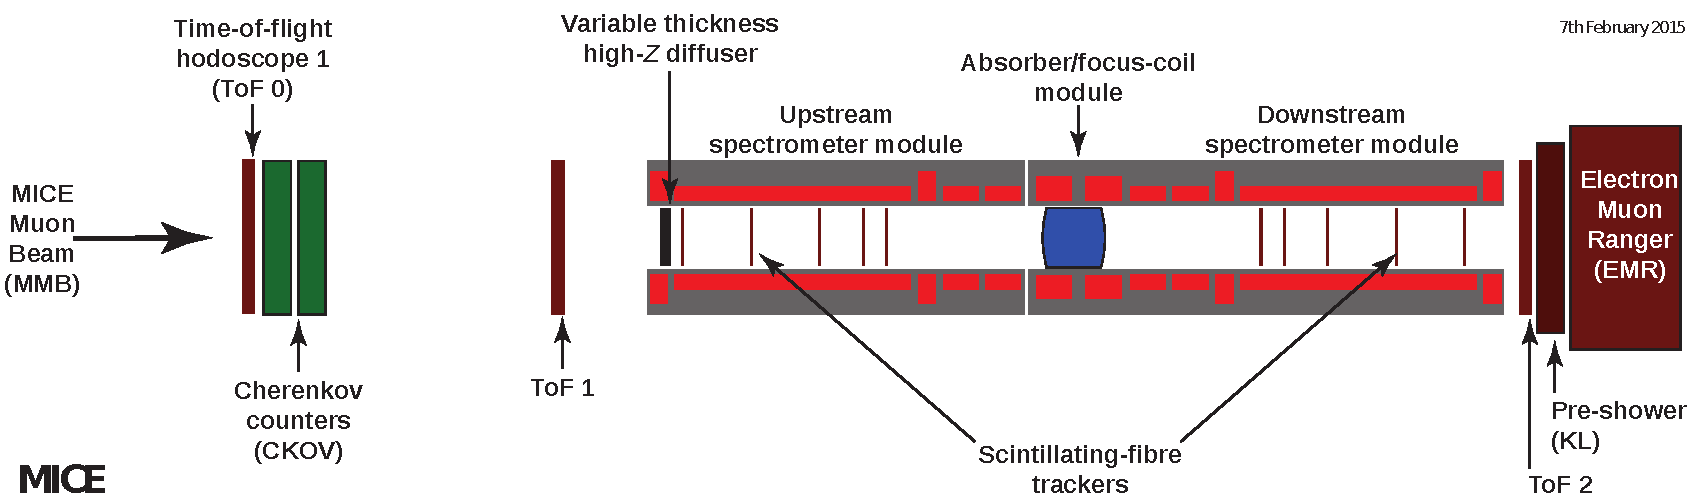
\includegraphics[width=0.9\textwidth]{Figures/mice}
}

%----------------------------------------------------------------------------------------
%	Stochastic Processes
%----------------------------------------------------------------------------------------
\headerbox{Stochastic Processes}{name=stochastic,column=0,row=1,below=mice}
{
The stochastic processes of interest are straggling (fluctuation about a mean energy loss) and multiple angular scattering \cite{icap15}.
Straggling follows Landau theory and has the form \cite{landau}
\begin{equation}
f(\lambda) = \frac{1}{\xi} \cdot \frac{1}{2\pi i} \int_{c+i \infty} ^{c-i \infty} \text{exp}(x\text{ ln } x + \lambda x) dx,
\label{eq:landau}
\end{equation}
where $\xi \propto Z\rho L/\beta^2 A$, and $\lambda \propto dE/\xi - \beta^2 - \text{ln } \xi$. Here $Z, A,$ and $\rho$ are the atomic charge, atomic mass, and density of the material; $L$ is the amount of material that the particle traverses; $\beta=v/c$; and $dE$ is the fluctuation about the mean energy. The algorithm based on Eq.~\eqref{eq:landau} has been implemented in COSY.

The derivation of the scattering function $g(u)$ (where  $u = \cos\theta$) is done separately for small angles and large angles. For small angles, the shape is very nearly Gaussian in $\theta$ \cite{GS}. For large angles, the distribution follows the Mott scattering cross section and is Rutherford-like \cite{Mott}. The resulting peak and tail are continuous and smooth at some critical $u_0$, which yields the final form of $g(u)$:
\begin{equation}
  g(u) = \left\{
  \begin{array}{lr}
    \displaystyle{\exp\left(-\frac{1}{2}\frac{1-u}{1-u_\sigma}\right)} & |\text{ } u_0 < u\vspace*{5pt}\\
%    \displaystyle{} \\
    \displaystyle{\zeta\cdot\frac{1+\frac{1}{2}(\beta\gamma)^2(1+u-b)}{(1-u+b)^2}} & | \text{ } u \le u_0
  \end{array}.
\right.
\label{eq:scattering}
\end{equation}
Here the parameters $\zeta$ and $b$ are chosen to ensure continuity and smoothness, $\gamma=1/\sqrt{1-\beta^2}$, $u_0$ is a fitted parameter, and $u_\sigma$ is the $\sigma$-like term for a Gaussian in $\theta$. It is another fitted parameter based on \cite{highland} and taking the form
\iffalse
\begin{footnotesize}
\[
u_\sigma=&\cos\left(\frac{13.6 \text{ MeV}}{\beta pc}\left(\frac{L}{L_0}\left(1+0.103\ln\frac{L}{L_0}\right)+0.0038\left(\ln\frac{L}{L_0}\right)^2\right)^\frac{1}{2}\right).
\]
\end{footnotesize}
\fi
\begin{align*}
u_\sigma=&\cos\Bigg(\frac{13.6 \text{ MeV}}{\beta pc}\Bigg(\frac{L}{L_0}\left(1+0.103\ln\frac{L}{L_0}\right)\\
&+0.0038\left(\ln\frac{L}{L_0}\right)^2\Bigg)^\frac{1}{2}\Bigg).
\end{align*}
}

%----------------------------------------------------------------------------------------
%	References
%----------------------------------------------------------------------------------------

\headerbox{References}{name=references,column=0,row=2,below=stochastic}
{
\renewcommand{\section}[2]{}% Gets rid of header
\bibliography{bib}{}
\bibliographystyle{plain}
}
%----------------------------------------------------------------------------------------
%	Absorbers
%----------------------------------------------------------------------------------------

\headerbox{Absorbers}{name=absorbers,column=1,row=1,below=mice}
{

Recently, COSY Infinity \cite{cosy} has been outfitted with new simulations tools for matter-dominated lattices \cite{ipac2015}, with the application of cooling absorbers as the motivation. Some of these results are reproduced here.
\\

Excellent agreement has been achieved between COSY, G4Beamline \cite{g4bl}, and ICOOL \cite{icool} for pencil beams of $p=$ (100, 200, 300, 400) MeV/$c$ through liquid hydrogen absorbers of lengths $L =$ (1, 10, 100) mm. Also, agreement has been shown with the MuScat results \cite{muscat}, with one example shown below.
\begin{center}
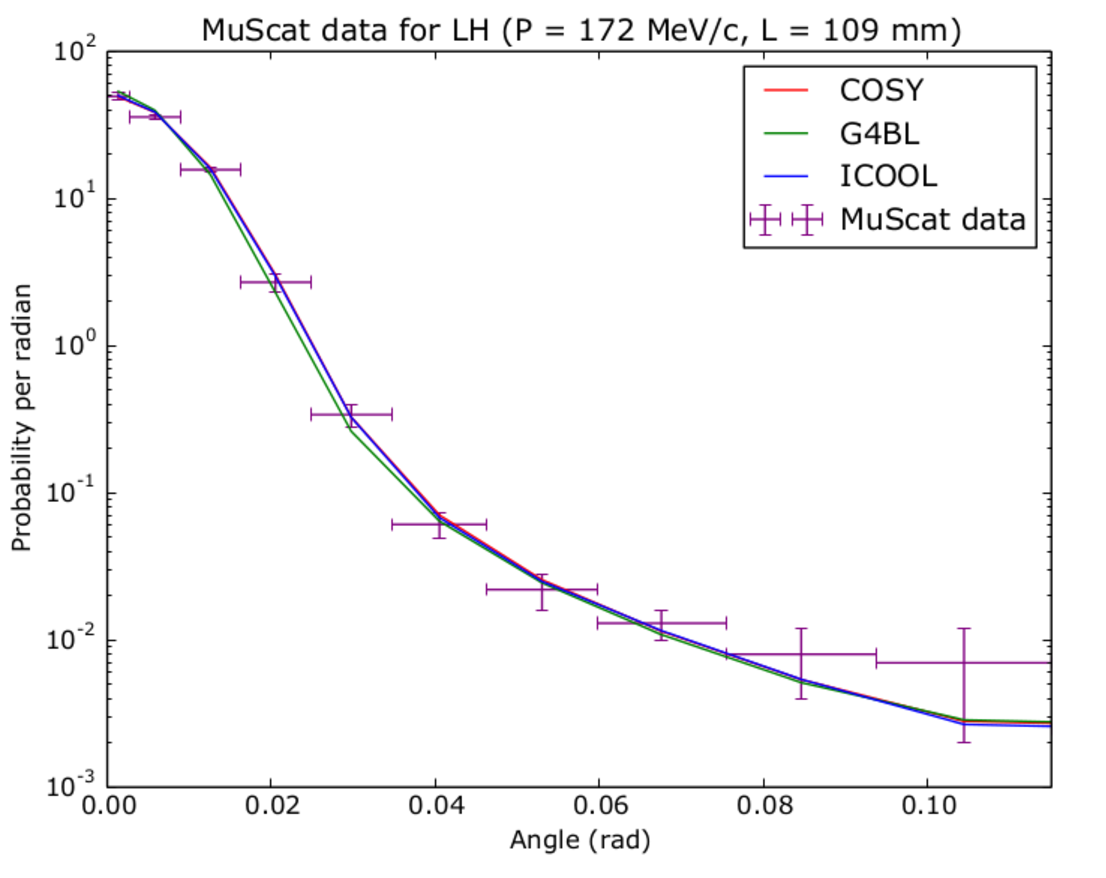
\includegraphics[width=0.9\textwidth]{Figures/Figure2poster}
%\caption{MuScat \cite{muscat} results for a collimated beam of muons of momenta 172 MeV/$c$ through 109 mm of liquid hydrogen.}
\end{center}
}

%----------------------------------------------------------------------------------------
%	MICE Cell
%----------------------------------------------------------------------------------------

\headerbox{The MICE cell}{name=micecell,column=1,row=1,below=absorbers}
{
MICE was simulated in-parts by COSY and G4Beamline. The initial distribution can be seen in the table below, along with the results of these separate simualtions.
%\begin{center} 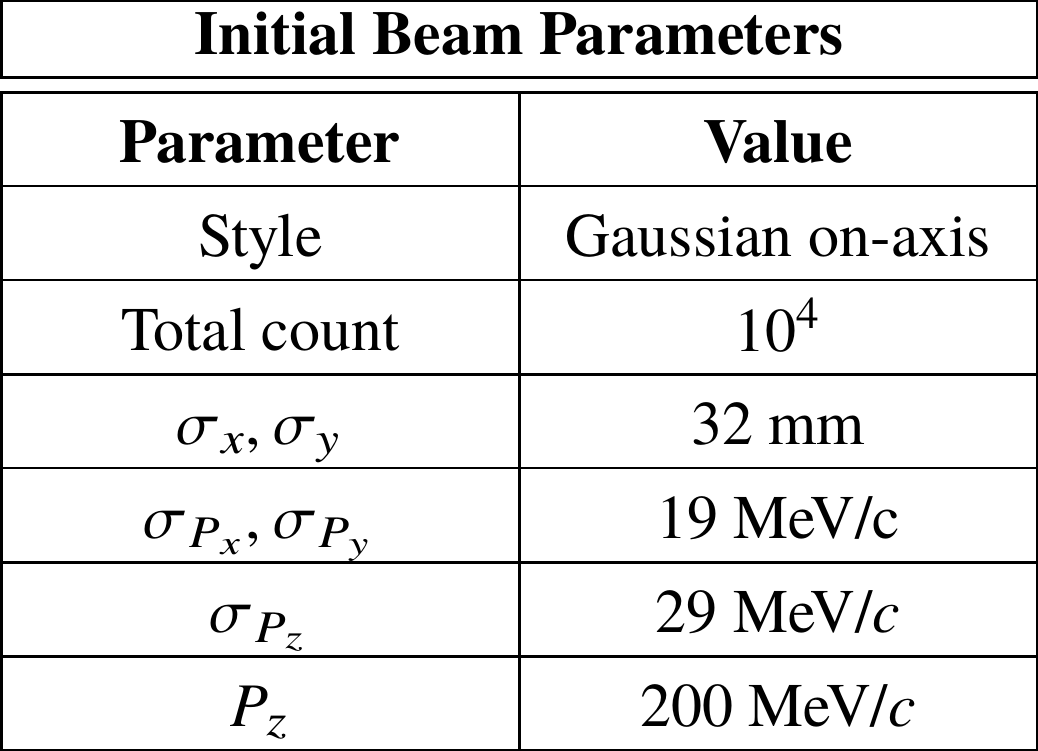
\includegraphics[width=0.73\textwidth]{Figures/initial_distribution_table} \end{center}
The absorber was a cylindrical lithium hydride block of 65 mm.\\
%\includegraphics[width=0.5\textwidth]{Figures/wedge tests (LiH)/xposition}\includegraphics[width=0.5\textwidth]{Figures/wedge tests (LiH)/xangle}
%\begin{center} \includegraphics[width=0.5\textwidth]{Figures/wedge tests (LiH)/energy} \end{center}
The coils (as seen in the MICE layout figure) were simulated to and from the scintillating-fibre trackers.\\
%\includegraphics[width=0.5\textwidth]{Figures/coil tests/xposition}\includegraphics[width=0.5\textwidth]{Figures/coil tests/xangle}
%\begin{center} \includegraphics[width=0.5\textwidth]{Figures/coil tests/energy} \end{center}
Coil parameters are summarized in the table below.
%\begin{center} 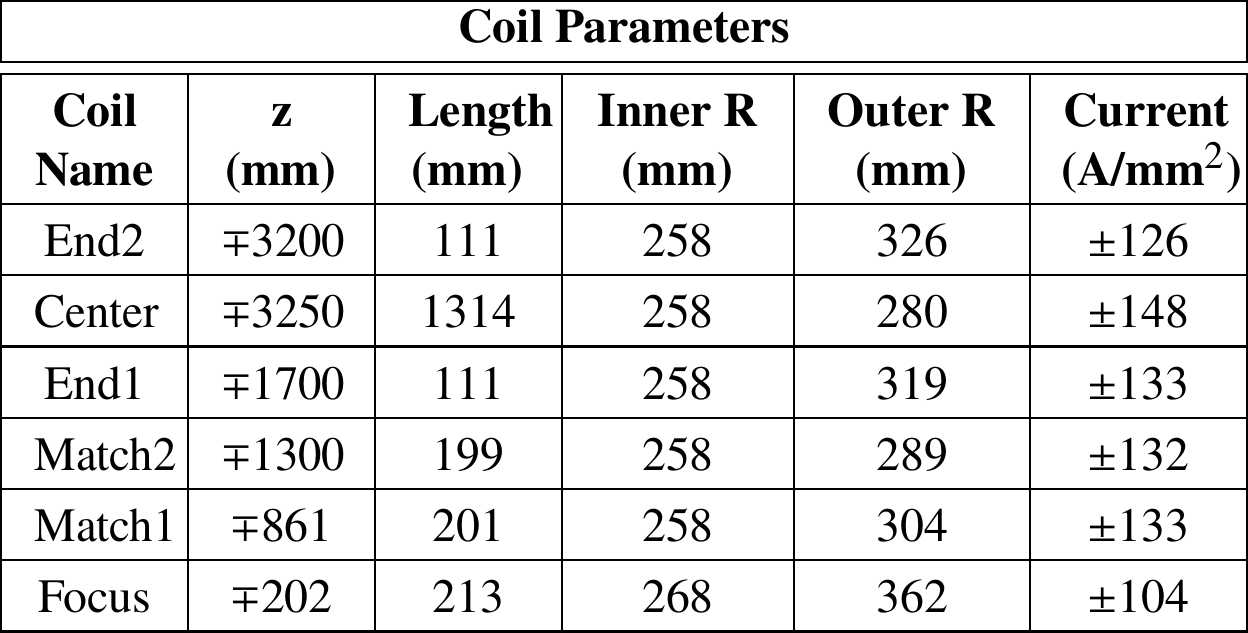
\includegraphics[width=0.95\textwidth]{Figures/coiltable} \end{center}
}

%----------------------------------------------------------------------------------------
% 	MICE Results
%----------------------------------------------------------------------------------------

\headerbox{MICE Results}{name=miceResults,column=2,row=0}
{
The results of the MICE simulation for 350 mm of liquid hydrogen are shown below.
\begin{center}
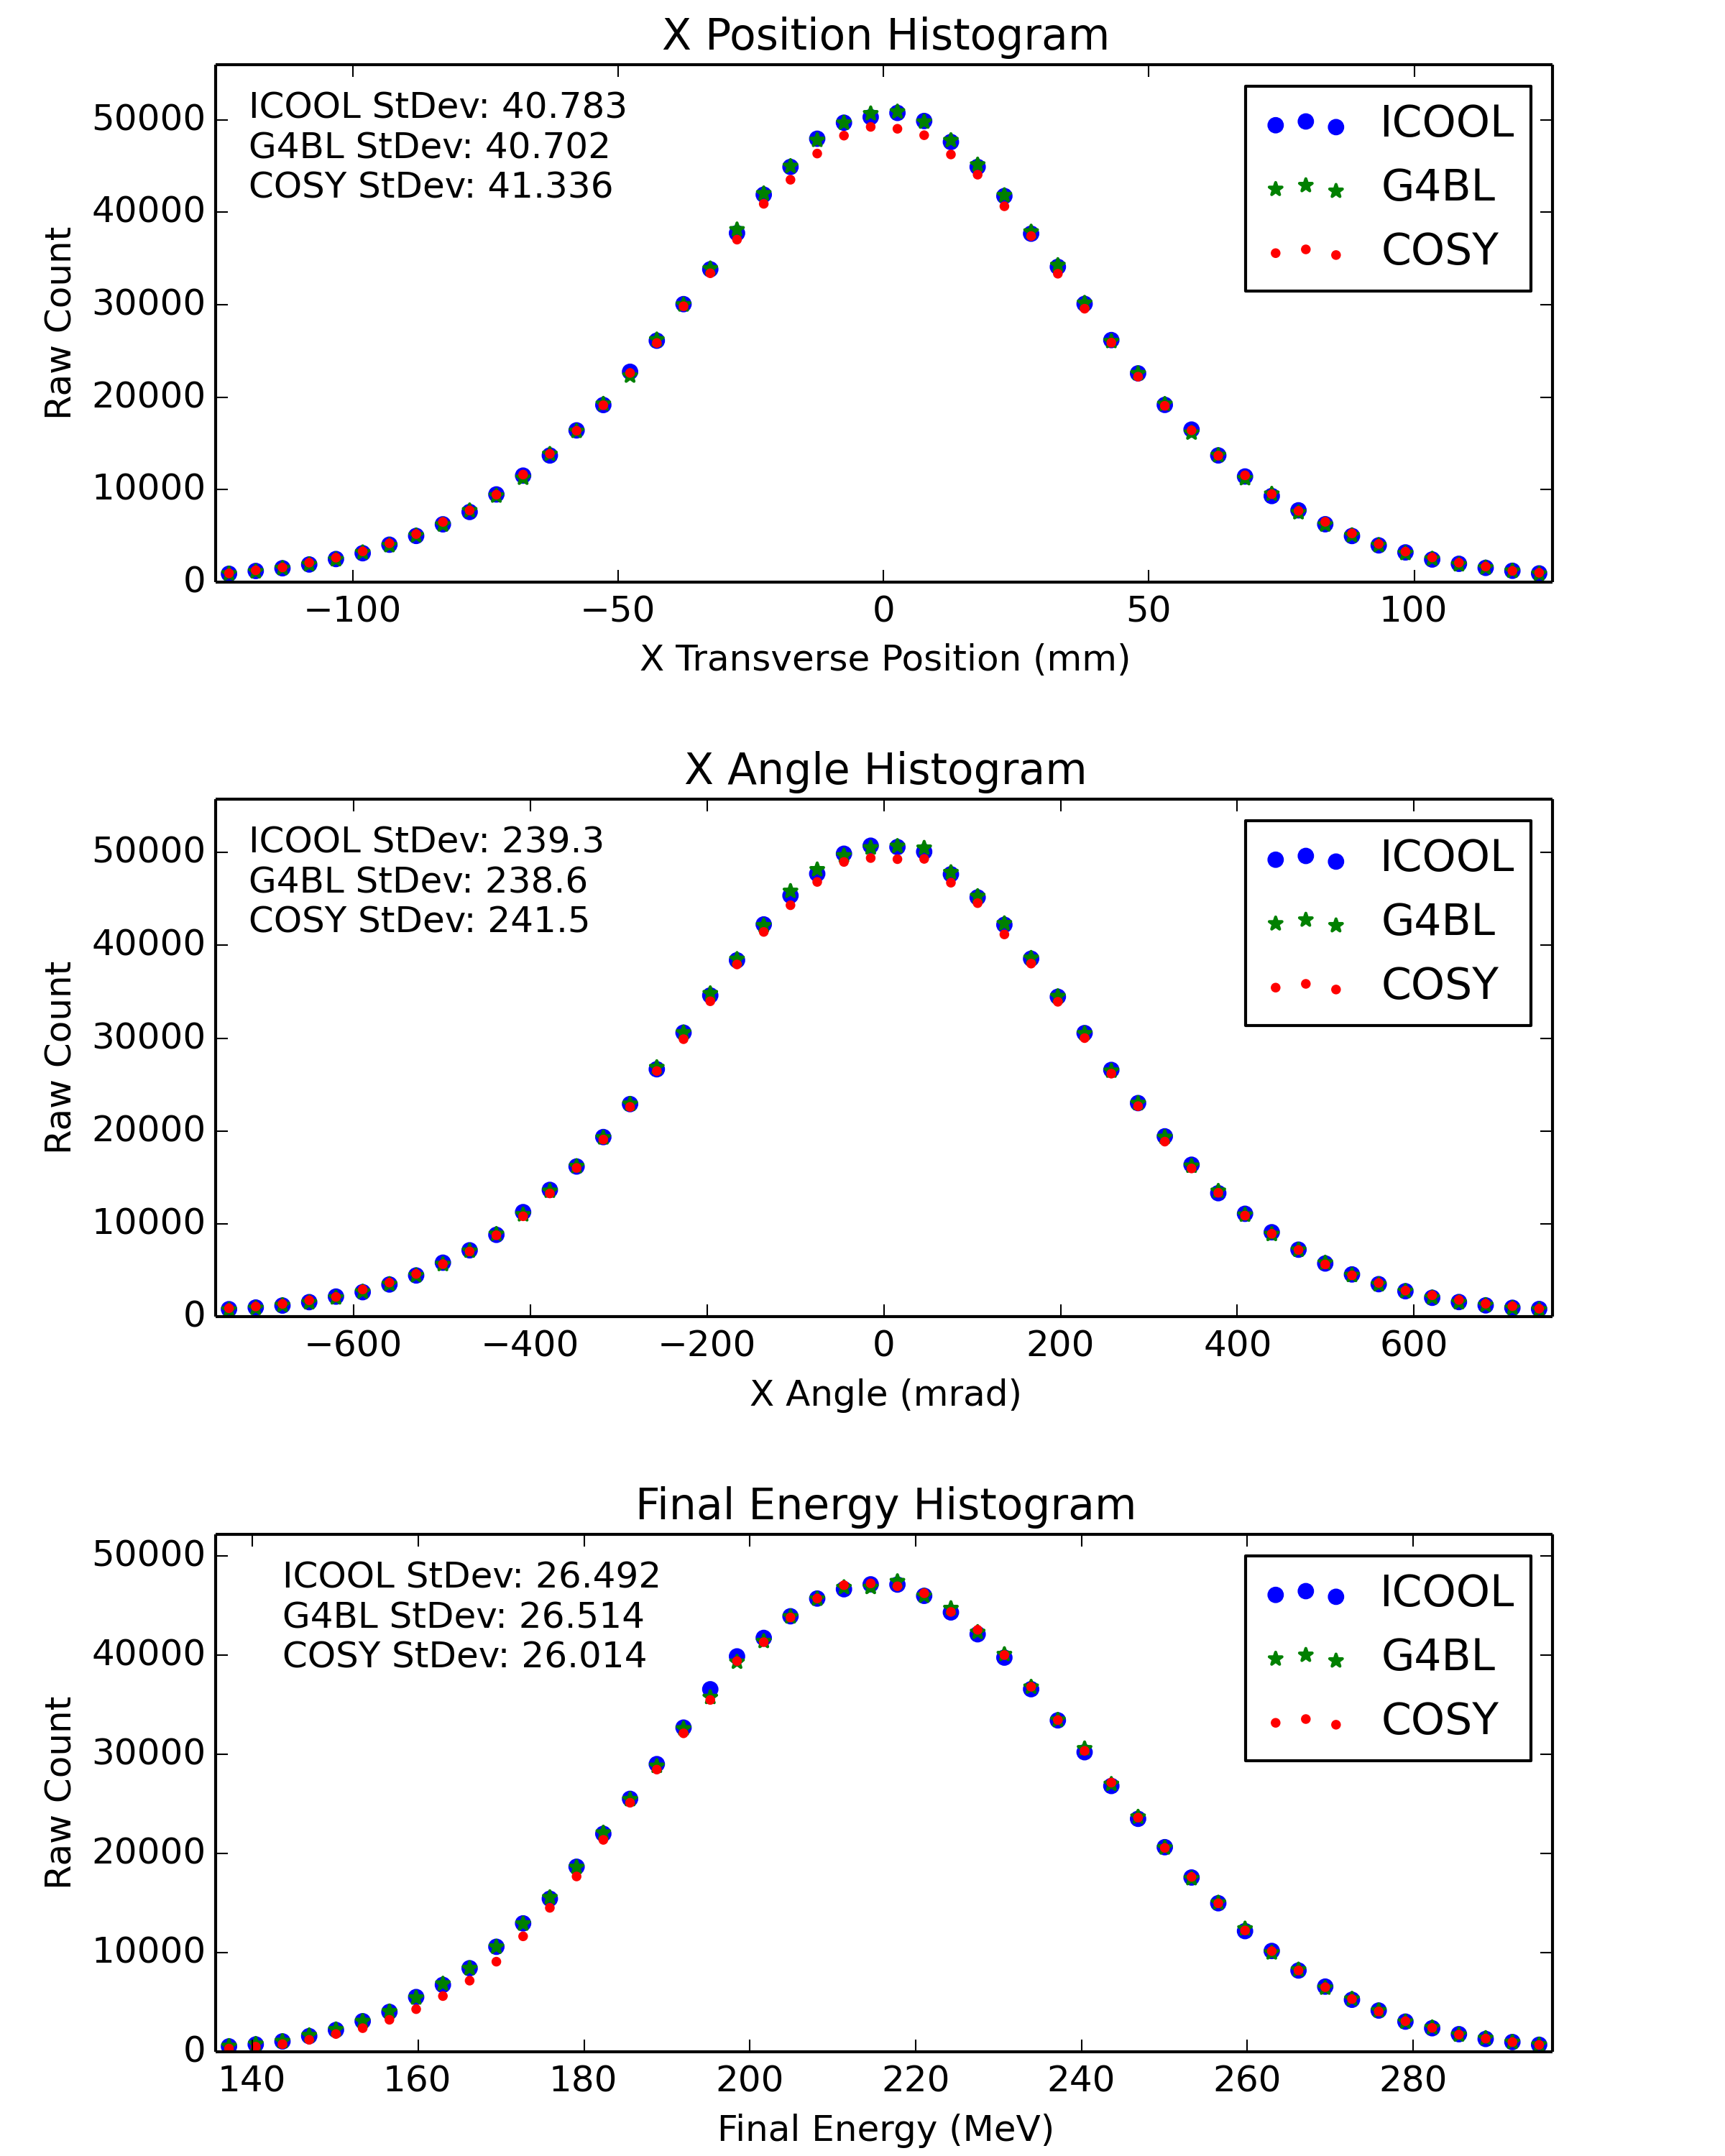
\includegraphics[width=\textwidth]{Figures/MICE_LH}
\end{center}

A simulation was also ran with 65 mm of lithium hydride. These results are shown below.

\begin{center}
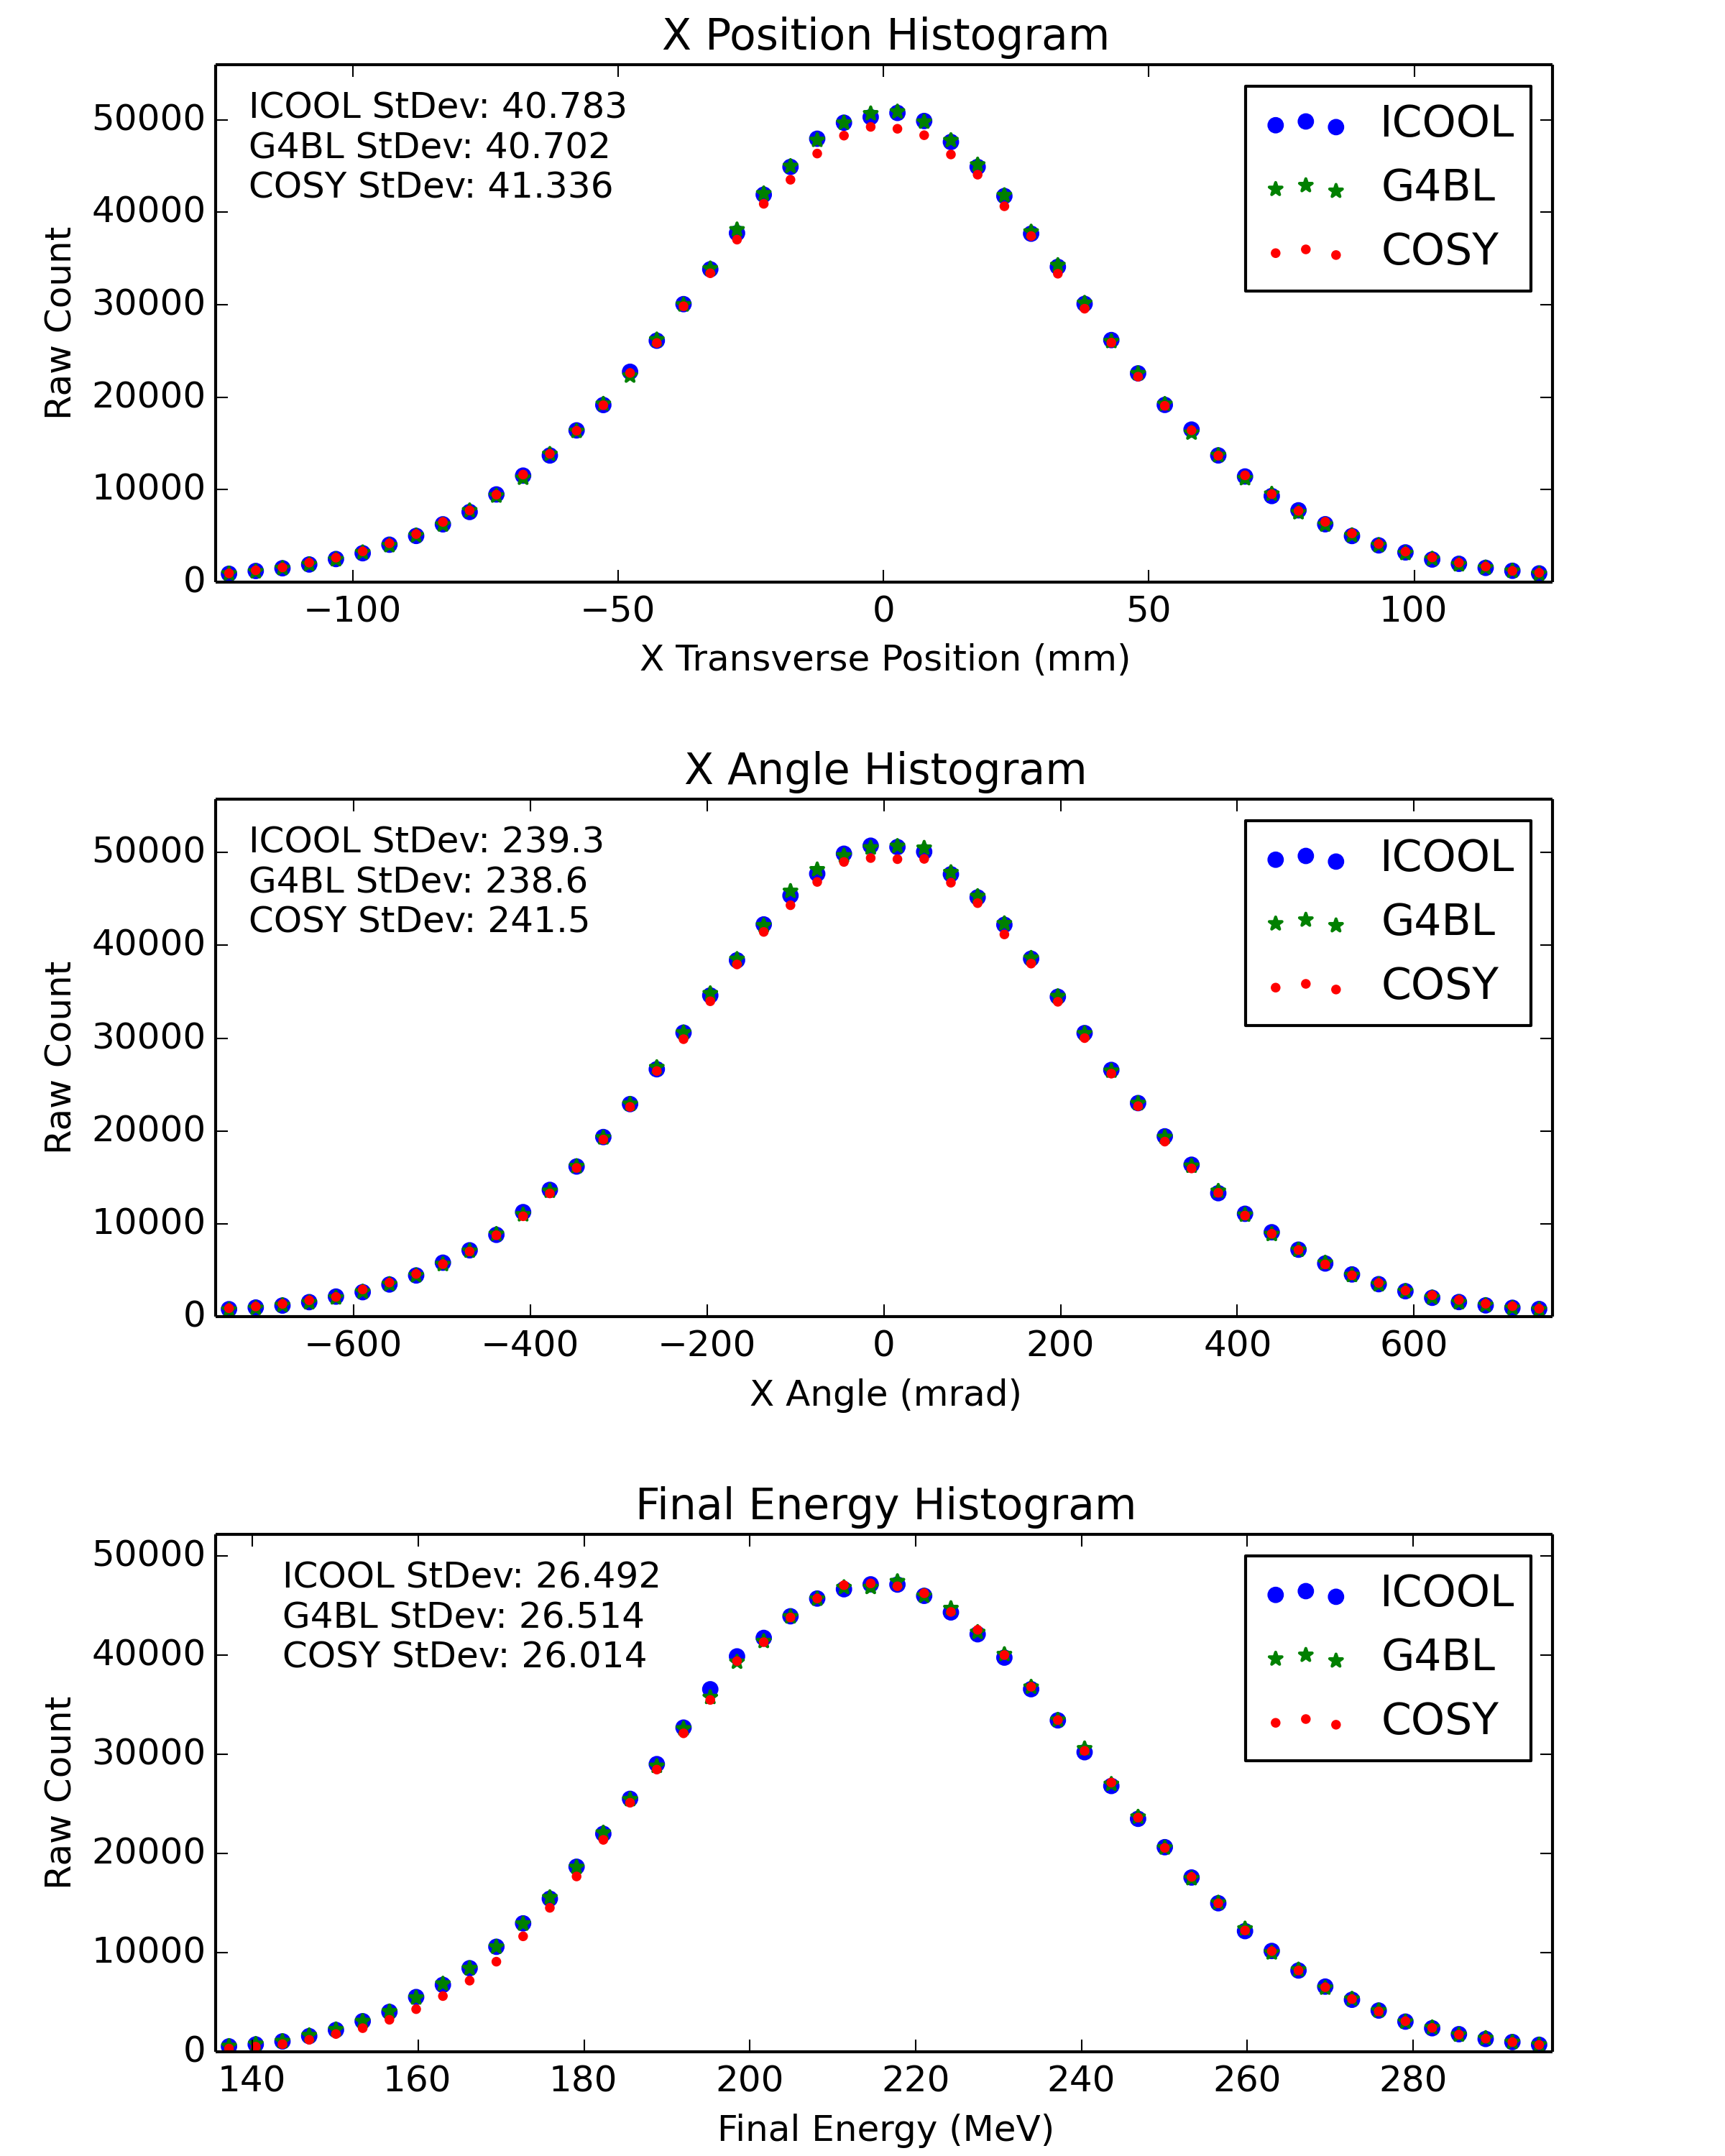
\includegraphics[width=\textwidth]{Figures/MICE_LH}
\end{center}

Computational times for liquid hydrogen can be seen in the following table. It can be concluded that the new hybrid approach in COSY is about twice as fast as G4Beamline and about three times as fast as ICOOL.
\iffalse
\begin{table}
%\caption*{\textbf{Run Times (in seconds) for MICE Step IV Simulation}}
\begin{center}
\begin{tabularx}{\columnwidth}{ccccc}
%\vspace{-40pt}\\ 
\hline \hline \vspace*{-10pt} \\
Number of particles: & $10^6$ & $10^5$ & $10^4$ & $10^3$\\
\hline
COSY: & 367 & 31 & 6 & 4\\
G4BL (coils): & 3973 & 392 & 40 & 6\\
G4BL (field map): & 662 & 75 & 15 & 9\\
ICOOL (field map): & 1091 & 117 & 19 & 9\\
\hline
\end{tabularx}
\end{center}
%\caption[Run times for MICE Step IV simulation.]{Run times for MICE Step IV simulation for liquid hydrogen. Note that the G4Beamline initialization time was not added to the run time values. G4BL (coils) represents the simulation in G4Beamline when the \texttt{coil} parameter was used. G4BL (field map) represents the simulation when G4Beamline (like ICOOL) read the field map from a file.}
%\label{tbl:mice_times}
\end{table}
\fi
}

\end{poster}

\end{document}